\chapter{Setup}
In this chapter, the setup and its components are introduced. 
First, the Citiroc 1A \ac{asic} and its evaluation board are presented. 
Then the used \ac{sipm} array is shown and in the last part of this chapter the box housing the \ac{sipm}s during the measurements is presented.



\section{Citiroc 1A}
Developed by the company Weeroc, the Citiroc 1A is an \ac{asic} for the readout of \ac{sipm}s. 
In essence, it is an amplifier and shaper for an input signal with trigger capabilities and a multiplexer output for the shaper signal amplitude.
So the charge signal coming from a \ac{sipm} gets amplified by the amplifier and integrated by the shaper.
The maximum of this integrated signal is than connected to a multiplexed output.
With this multiplexed output, all channels can be read out one after another at the same output of the Citiroc 1A.
Therefore the number of \acp{adc} needed to digitize the signals from every channel is reduced by a factor of 31.
A sketch of the internal electronics of the Citiroc 1A is shown in \autoref{fig:citiroc1a_sketch}.

\begin{figure}
    \centering
    \includegraphics[width=1.\textwidth]{citiroc/citiroc}
    \caption[Citiroc 1A sketch]{Depiction of the main components of the Citiroc 1A. 
	The 32 channels with the inputs and the input DACs are followed by a low and a high gain preamplifier. 
	Both amplified signals are shaped by slow shapers and the peak sensing cell returns the shaper signal amplitude to a multiplexer common to all channels. 
	Also, the trigger part with a fast shaper followed by two discriminators is shown. 
	One discriminator output is connected to a common multiplexer and an OR of the 32 channels. 
	The other discriminator is connected to a channel by channel time trigger output and also to a common OR. 
	The trigger threshold of both discriminators can be set individually but common for all channels via a 10-bit DAC. \cite{citiroc}}
    \label{fig:citiroc1a_sketch}
\end{figure}

The Citiroc 1A has 32 channels. 
Each channel has an 8-bit input \ac{dac} which allows tuning the high voltage on a channel by channel level.
When the high voltage $V_\text{HV}$ is supplied to the \ac{sipm}s and the \ac{dac} voltage is $V_\text{DAC}$ the bias voltage on the \ac{sipm}s is
\begin{align}
	V_\text{bias} &= V_\text{HV} - V_\text{DAC}.
\end{align}
The input \ac{dac}s are connected to the inputs with resistors in series, so that the fast charge signal from the \ac{sipm}s is not disturbed by the input \ac{dac}.
Besides the 32 inputs, one \textit{IN\_CALIB} input exists with which a signal can be injected into one of the 32 channels.
The injected signal goes over a \SI{3}{\piko\farad} capacitor into the preamplifier.
A sketch of this is shown in \autoref{fig:citiroc_amp}.
After the input, there are two amplifiers in parallel.
One high gain amplifier and one low gain amplifier so that a broader input range can be covered.
The structure of both amplifiers is the same and shown in \autoref{fig:citiroc_amp}.
They each have a capacitor $\text{C}_\text{in}$ in series and then a variable feedback capacitor $\text{C}_\text{f}$ in parallel, which can be set to values from \SIrange{0}{1575}{\femto\farad} in \SI{25}{\femto\farad} steps.
The capacitors connected in series have fixed capacitances.
The low gain preamplifier capacitor has \SI{1.5}{\piko\farad} and the high gain preamplifier has a \SI{15}{\piko\farad} capacitance.
The Citiroc 1A datasheet states that the resulting amplification can be calculated with
\begin{align}
	AMP &= \frac{\text{C}_\text{in}}{\text{C}_\text{f}}.
\end{align}
Since this equation is not defined for $\text{C}_\text{f}=\SI{0}{\femto\farad}$, that value was not used for the measurements in this thesis.
For the other possible feedback capacitor values the resulting high gain and low gain amplifications are \SIrange[per-mode=symbol]{9.5}{60}{\volt\per\volt} and \SIrange[per-mode=symbol]{0.95}{6}{\volt\per\volt}, respectively. 
Each amplifier output is connected to a slow shaper and in addition one of the outputs can be connected to the trigger block of the Citiroc 1A.

\begin{figure}
	\centering
	\includegraphics[width=0.5\textwidth]{citiroc/preamp}
	\caption[Sketch of the Citiroc 1As preamplifiers]{Illustration of the preamplifiers in the Citiroc 1A. The signal is injected either through the IN input or through the IN\_Calib input. By changing the capacitance of the feedback capacitor, the gain can be set. \cite{citiroc}}
	\label{fig:citiroc_amp}
\end{figure}


\paragraph{The trigger unit} starts with the shaping of the amplifier output connected to the trigger unit. 
This is done by a CRRC fast shaper with a \SI{15}{\nano\second} peaking time \cite{citiroc}. 
The high pass filter of the fast shaper consists of a $C_\text{in}=\SI{5}{\piko\farad}$ capacitor and a $R_\text{in}=\SI{500}{\ohm}$ resistor.
The low pass filter constists of a $C_\text{f}=\SI{100}{\femto\farad}$ capacitor and a $R_\text{f}=\SI{25}{\kilo\ohm}$ resistor.
In \autoref{fig:fast_shaper} the schematics of the fast shaper are shown.
After the shaping, the signal goes into two discriminators.
By using the two 10-bit \ac{dac}s and the 4-bit \ac{dac}s, also connected to the discriminator, a trigger threshold can be set.
While the two 10-bit \ac{dac}s are common for all the 32 channels, each channel has its own two 4-bit \ac{dac}s.
This allows to fine-tune the common threshold set by the 10-bit \ac{dac}s on a channel by channel level.
The time discriminator output is connected to an open-collector NOR of all 32 channels and can also be read out channel by channel, enabling the setting of time stamps for each channel.
The charge discriminator is followed by masking opting, which allows the channel by channel masking of the charge trigger. 
After the masking option, the charge trigger signal is connected to an OR of the 32 channels which can be read out as an OR or as an open-collector NOR.
The charge trigger can also be connected to a multiplexed output of all channels.
With this output, one can easily see in the measurement data which channel was triggered in each event.
Both triggers are sensitive down to 1/3 of a photoelectron \cite{citiroc}.

\begin{figure}
	\centering
	\includegraphics[width=.5\textwidth]{citiroc/fast_shaper}
	\caption[Citiroc 1A fast shaper schematic]{The fast shaper of the Citiroc 1A with the $\SI{5}{\piko\farad}$ capacitor $\text{C}_\text{in}$ and the $\SI{500}{\ohm}$ resistor $\text{R}_\txt{in}$ functioning as high pass filter. The capacitor $\text{C}_\text{f}=\SI{100}{\femto\farad}$ and the resistor $\text{R}_\text{f}=\SI{25}{\kilo\ohm}$ working as a low pass filter. The resulting peaking time is $t_\test{peak}=\SI{15}{\nano\second}$. \cite{citiroc}}
	\label{fig:fast_shaper}
\end{figure}


\paragraph{For the charge measurement} the outputs of the two preamplifiers are connected to two CRRC$^2$ slow shapers, depicted in \autoref{fig:slow_shaper}.
The time constant for the high pass filter and the two low pass filters can be set from \SIrange{12.5}{87.5}{\nano\second} in \SI{12.5}{\nano\second} steps.
This results in an overall peaking time of \SIrange{25}{175}{\nano\second} in \SI{25}{\nano\second}.
\begin{figure}
	\centering
	\includegraphics[width=1.\textwidth]{citiroc/slow_shaper}
	\caption[Citiroc 1A slow shaper schematic]{Schematic of the Citiroc 1As CRRC$^2$ slow shapers. Each CR or RC part has a time constant changeable from \SIrange{12.5}{87.5}{\nano\second} in \SI{12.5}{\nano\second} by changing the capacitance of the capacitors. \cite{citiroc}}
	\label{fig:slow_shaper}
\end{figure}
The slow shapers are followed by a peak sensing cell which gives the maximum shaper amplitude out to a multiplexer.
Two options for finding the amplitude to put out are built in the peak sensing cell.
The first option is the \textit{SCA} which works with the \textit{sample and hold} method.
It recuires an external \testit{hold} signal.
The SCA tracks the shaper output constantly, until the external hold signal rises from low to high.
On the rising edge of the hold signal, it samples the shaper amplitude and holds it until the hold signal falls back to low.
In order to sample the maximum of the shaper amplitude, the rising edge of the hold signal must arrive, when the shaper signal is at its maximum. 


The second peak sensing option is the \textit{peak detector}.
It starts in an idle phase and upon an arriving trigger, the internal charge trigger or an external trigger, it starts tracking the maximum of the shaper amplitude.
When the external hold signal rises to high, the maximum amplitude is held, as long as the hold signal is high.
During that time, the amplitude can be read out via the multiplexer.
When the hold signal falls back to low, the peak detector enters the idle phase again.

The trigger starting the peak sensing tracking phase as well as the hold signal required for the peak sensing and the SCA are both common to all 32 channels.
While the amplitudes of all channels are held, the three multiplexers put out the low gain amplitude, the high gain amplitude, and the charge trigger, one channel after another.
The multiplexer requires an external clock signal to shift between the channels. 
In order to achieve a 10-bit resolution on the output, the clock's frequency should be less than \SI{5}{\mega\hertz}.
This leads to a readout time per channel of at least \SI{200}{\nano\second} and a total readout time of more than \SI{6.4}{\micro\second}.
Since the Citiroc 1A holds the shaper amplitude during that time, it is blind to other events happening while the read-out of the multiplexed output is going on.
Therefore a continuous readout is not possible with the Citiroc 1A.


In order to simplify working with the Citiroc 1A and getting to know it, the Citiroc 1A evaluation board was used.
It is presented in the following section.








\subsection{Citiroc 1A evaluation board}

To make it easier to work with the Citiroc 1A, the corresponding evaluation board houses everything necessary except a computer to operate the Citiroc 1A.
A picture of the Citiroc 1A evaluation board is shown in \autoref{fig:citiroc_evaluation_board}.
In the center of the evaluation board is the Citiroc 1A \ac{asic} placed.
Next to it are 32 pairs of pins for connecting the \ac{sipm}s.
One row is connected to the 32 inputs of the Citiroc 1A and the other one can be used to supply the \ac{sipm}s via the evaluation board with high voltage.
For this purpose, a connector can be soldered on the evaluation board over which the board can be supplied with the high voltage for the \ac{sipm}s.
Over an SMA connector signals can be injected into the Citiroc 1As IN\_CALIB input.
Via three SMA connectors, the analog probes of the Citiroc 1A can be read out.
With two onboard 12-bit \ac{adc}s to read out the low gain and high gain multiplexer outputs of the Citiroc 1A.
Optional one of the \ac{adc}s can be used to digitize a test signal which can be injected into the \ac{adc} over a connector on the evaluation board.
The other \ac{adc} can also be used to read out the temperature probe in the Citiroc 1A.
For processing the digitized measurement data an FPGA is placed on the evaluation board.
The firmware for the FPGA as well as the slow control parameters for the Citiroc 1A can be provided via the USB interface.
This interface can also be used to supply the evaluation board with power instead of using the power connector on the board.
In order to operate the Citiroc 1A evaluation board, Weeroc developed a computer program for the Windows operating system.
With this program, the Citiroc 1A slow control parameter can be chosen and sent to the \ac{asic} as well as some FPGA settings.
The most important FPGA settings are the trigger settings, meaning which signal from the trigger block of the Citiroc 1A is used to trigger an event and the time delay between the arrival of the trigger signal and the sending of the hold signal for the peak sensing cell.

The evaluation board also provides multiple FPGA input/outputs.
With these, for example, the digital trigger signal can be read out or a clock on the evaluation board can be put out and connected as a trigger to a light source.


In the following section, the \ac{sipm} array which was read out with the Citiroc 1A evaluation board is presented. 



%Since, due to ground loops, an external power supply introduced a lot of noise into the measurements, a Laptop was used to supply the power via the USB interface. 
%This laptop was also used for loading the slow control and the FPGA firmware onto the evaluation board and storing the measurement data.
%One FPGA input/output can be used to probe the digital outputs, e.g. the OR trigger of a single channel, of the Citiroc 1A.

\begin{figure}
    \centering
    \includegraphics[width=1.\textwidth]{citiroc/citiroc_evaluation_board.jpg}
    \caption{The Citiroc 1A evaluation board with the Citiroc 1A \ac{asic}, the 32 input pins, the probe outputs, two \ac{adc}s, one FPGA with its input/output connectors, and the USB interface.}
    \label{fig:citiroc_evaluation_board}
\end{figure}










\section{Silicon Photomultiplier Array}
The \ac{sipm} array that was used for the measurements consists of forty \textit{Hamamtsu S14160-3050HS} \ac{sipm}s which were soldered in a circle onto the \ac{pcb} shown in \autoref{fig:hamamatsu_pcb_front} and \autoref{fig:hamamatsu_pcb_back}.
In \autoref{tab:sipm_specs} are the specifications of these \ac{sipm}s listed.
The \ac{sipm}s were placed in a \SI{6}{\centi\meter} outer diameter circle onto the \ac{pcb}.
The connections on the \ac{pcb} were made so that the \ac{sipm}s are connected parallel in groups of five.
Each group has a dip switch with five switches placed between the \ac{sipm}s and the high voltage.
Therefore every individual \ac{sipm} can be turned on and off, simplifying debugging and allowing the examination of the signal difference between different numbers of \ac{sipm}s in parallel.
The circuit diagram of one example \ac{sipm} group is shown in \autoref{fig:hamamatsu_pcb_circuit}. 

\begin{figure}
	\centering
	\includegraphics[width=0.5\textwidth]{pictures/sipm_pcb}
	\caption[Circuit diagram of the connections on the \ac{sipm} \ac{pcb}]{Circuit diagram of the connections on the \ac{sipm} \ac{pcb} for one group of five \acp{sipm}. Each \ac{sipm} can be disconnected from the high voltage via a switch. The high voltage side of the \acp{sipm} is connected to ground over a \SI{100}{\nano\farad} capacitor.}
	\label{fig:hamamatsu_pcb_circuit}
\end{figure}

In order to connect the \ac{sipm} outputs to the Citiroc 1A evaluation board inputs and to supply the \ac{sipm}s with high voltage, a breakout board was used.
It can be connected to the back of the \ac{sipm} \ac{pcb}.
On the back of the breakout board are eight SMA connectors for the signal output of eight \ac{sipm} groups and one SMA connector for the common high voltage supply.
A picture of the breakout board is shown in \autoref{fig:hamamatsu_breakout}.



In order to be able to control the light exposure of the \ac{sipm}s during the measurements, they were placed inside of a light-tight box, which is described in the following chapter.

\begin{figure}
    \centering
    \begin{subfigure}[t]{0.33\textwidth}
        \centering
        \includegraphics[width=.95\linewidth]{pictures/hamamatsu_sipm_pcb_front.jpg}
        \caption{The \ac{pcb} front of the \ac{pcb}.}
        \label{fig:hamamatsu_pcb_front}
    \end{subfigure}%
    \begin{subfigure}[t]{0.33\textwidth}
        \centering
        \includegraphics[width=.95\linewidth]{pictures/hamamatsu_sipm_pcb_back.jpg}
        \caption{The back of the \ac{pcb}}
        \label{fig:hamamatsu_pcb_back}
    \end{subfigure}%
    \begin{subfigure}[t]{0.33\textwidth}
        \centering
        \includegraphics[width=.95\linewidth]{pictures/hamamatsu_breakout_on_sipm.jpg}
        \caption{The breakout board}
        \label{fig:hamamatsu_breakout}
    \end{subfigure}
	\caption[Hamamatsu \ac{sipm} array and the breakout board.]{The \ac{pcb} with the forty Hamamtsu S14160-3050HS \ac{sipm}s. 
	The \ac{sipm} circle has an outer diameter of \SI{6}{\centi\meter} (a). 
	On the back of the \ac{pcb} the eight dip switches are placed and the connector is soldered in the middle of the back (b). 
	Via the SMA connectors on the breakout board, the \ac{sipm}s can be supplied with power and the signals can be read out (c).}
\end{figure}





\begin{table}[]
    \centering
    \caption[Hamamatsu S14160-3050HS SiPM specifications]{Specifications of the \textit{Hamamatsu S14160-3050HS} \ac{sipm}s. \cite{HAMsipm_ds}}
    \setlength\extrarowheight{2.5pt}
    \begin{tabular}{lc}\toprule
	\ac{sipm} type & \textit{S14160-3050HS}  \\[2.5pt]\midrule
        Effective photosensitive area [\si{\square\milli\meter}] & $3.0\times 3.0$  \\[2.5pt]
        Pixel pitch [\si{\micro\meter}] & 50 \\[2.5pt]
        Number of pixels & 3531  \\[2.5pt]
        Window material & Silicone  \\[2.5pt]
        Window refractive index & 1.57  \\[2.5pt]\bottomrule
    \end{tabular}
    \label{tab:sipm_specs}
\end{table}



\section{Dark box}
A aluminum box was used to place the \ac{sipm} \ac{pcb} in and block the unwanted light from the surroundings from reaching the \ac{sipm}s.
On the inside, it was covered with black aluminum foil by Thorlabs \cite{thorlabs_aluminium}, with a reflectivity of less than \SI{5}{\percent} for light in the visible spectrum.
By this, the probability of photons entering the box to hit the \ac{sipm}s was decreased.
In addition, the weak points of the box for which the light tightness can not be guaranteed were covered with multiple layers of tape.

Multiple SMA, SMC, and BNC feedthroughs were added for high voltage and signal transfer in and out of the box.
Another self-made fiber feedthrough was used to lay two optical fibers stable from the outside into the box without causing light leaks. 
The two fibers were used for guiding the light from a LED and a Laser into the box.

To fix the \ac{sipm} \ac{pcb} in place the optical rail was used. 
Besides the \ac{sipm} array also mounts for the two optical fibers as well as a diffuser \cite{thorlabs_diffusor} could be mounted if needed for a measurement.

To further decrease the probability of light leaks an optical blanket was used to cover the box after closing and the room was darkened during the measurements.

In the last part of this chapter, the LED used as a light source in this thesis is presented.

\begin{figure}
	\centering
	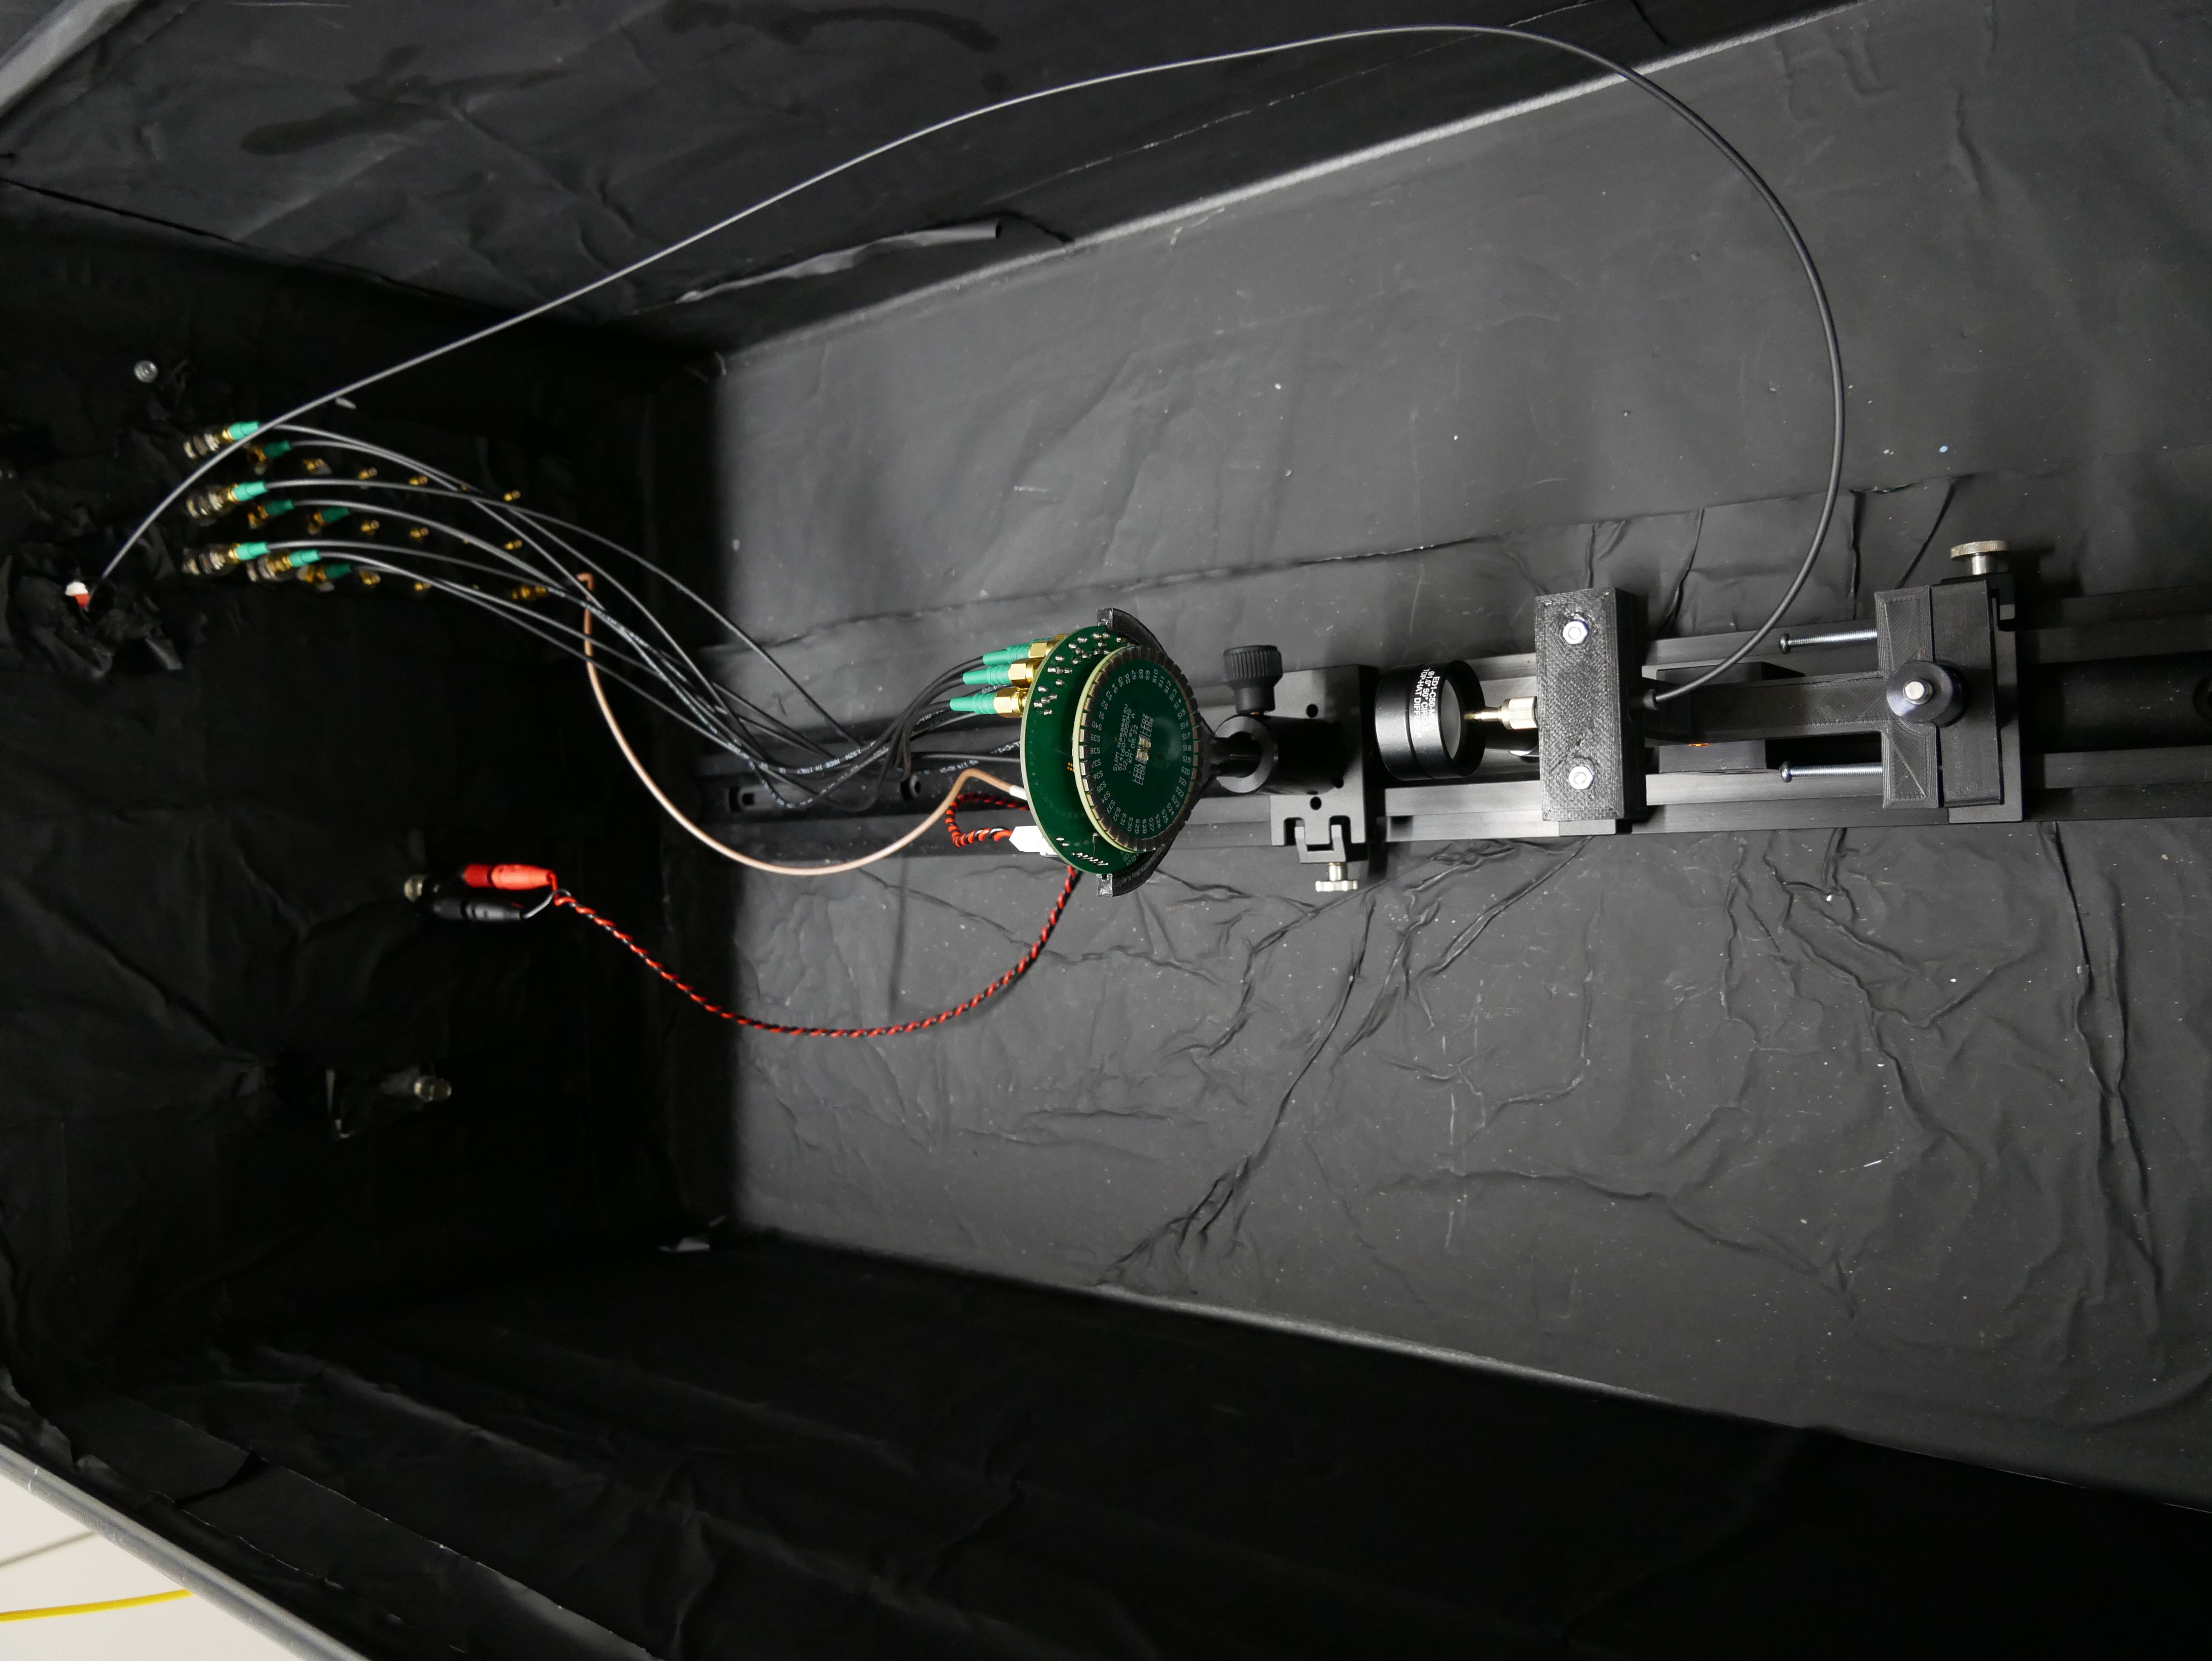
\includegraphics[width=1.\textwidth]{pictures/setup_box_pic}
	\caption[Setup inside the aluminum Box]{The setup inside the aluminum box with the \ac{sipm} array, the diffusor and the fiber coming from the LED.}
	\label{fig:setup_inside_box}
\end{figure}



\section{Light sources}
To have a controlled light exposure a \SI{460}{\nano\meter} LED setup was used.
This setup was built in the bachelor thesis by Alexander Bismark \cite{alex_bismark}.
It consists of a small light-tight box with a LED inside, which is connected to a BNC feedthrough.
Via a waveform generator connected to the BNC feedthrough the LED can be supplied with voltage pulses adjustable in length and amplitude. 
One end of an optical fiber is placed inside the LED box to capture a small part of the light emitted by the LED.
The other end of the SMA terminated fiber is outside of the LED box and fed into and mounted inside of the aluminum box with the \ac{sipm}s.
By using a diffusor by Thorlabs \cite{thorlabs_diffusor} multiple \ac{sipm}s can be exposed to the light at the same time. 

For the measurements in this thesis which used the LED the length of the voltage pulses was set to \SI{10}{\nano\second} with a rise time and fall time of \SI{2.5}{\nano\second}.
The amplitude of the pulses was adjusted to achieve the desired light exposure.

\mbox{}

\mbox{}

In \autoref{fig:setup_inside_box} a sketch of the complete assembled setup is shown.
The \acp{sipm} were placed inside the box and supplied with high voltage from the outside of the box by a high voltage supply.
The signal outputs of the \acp{sipm} are connected to the Citiroc 1A evaluation boards inputs.
A laptop was used to load the slow control for the Citiroc 1A on the evaluation board, to save the data measured by the evaluation board and to supply power to the evaluation board.
With the waveform generator supplying the LED with voltage pulses for it to emit the light which was guided inside the aluminum box.
In the aluminum box a diffusor ensured even light exposure of the whole \ac{sipm} array.

In the next chapter the measurements performed with this setup are presented.


\begin{figure}
	\centering
	\includegraphics[width=1.\textwidth]{pictures/setup_box}
	\caption[Illustration of the measurement setup]{Illustration of the setup used for the measurements. The \acp{sipm} array was placed inside the aluminum box to shield it from unwanted light. A power supply was used to supply the \acp{sipm} with high voltage. The signal outputs from the \ac{sipm} array were connected to the inputs of the Citiroc 1A evaluation boards inputs. The data processed on the evaluation board was send to the laptop for storage. The laptop also provided the power for the evaluation board and was used to control the Citiroc 1A and load the slow control for it onto the evaluation board. With the waveform generator a LED was pulsed and the emitted light was guided into the aluminum box and there diffused for an even light exposure of the \acp{sipm}.}
	\label{fig:setup_inside_box}
\end{figure}
